% This template was initially provided by Dulip Withanage.
% Modifications for the database systems research group
% were made by Conny Junghans,  Jannik Strötgen and Michael Gertz

\documentclass[
     12pt,         % font size
     a4paper,      % paper format
     BCOR10mm,     % binding correction
     DIV14,        % stripe size for margin calculation
     ]{article}

%%%%%%%%%%%%%%%%%%%%%%%%%%%%%%%%%%%%%%%%%%%%%%%%%%%%%%%%%%%%

% PACKAGES:

% Use German :
\usepackage[english]{babel}
% Input and font encoding
\usepackage[latin1]{inputenc}
\usepackage[T1]{fontenc}
% Index-generation
\usepackage{makeidx}
% Einbinden von URLs:
\usepackage{url}
% Special \LaTex symbols (e.g. \BibTeX):
%\usepackage{doc}
% Include Graphic-files:
\usepackage{graphicx}
% Include doc++ generated tex-files:
%\usepackage{docxx}

% Fuer anderthalbzeiligen Textsatz
\usepackage{setspace}

% hyperrefs in the documents
\PassOptionsToPackage{hyphens}{url}\usepackage[bookmarks=true,colorlinks,pdfpagelabels,pdfstartview = FitH,bookmarksopen = true,bookmarksnumbered = true,linkcolor = black,plainpages = false,hypertexnames = false,citecolor = black,urlcolor=black]{hyperref}
%\usepackage{hyperref}

%%%%%%%%%%%%%%%%%%%%%%%%%%%%%%%%%%%%%%%%%%%%%%%%%%%%%%%%%%%%

% OTHER SETTINGS:

% Choose language
\newcommand{\setlang}[1]{\selectlanguage{#1}\nonfrenchspacing}


\begin{document}

% TITLE:
\pagenumbering{roman} 
\begin{titlepage}


\vspace*{1cm}
\begin{center}
\vspace*{3cm}
\textbf{ 
\Large Heidelberg University\\
\smallskip
\Large Institute of Computer Science\\
%\smallskip
%\Large Database Systems Research Group\\
\smallskip
}

\vspace{3cm}

\textbf{\large Project Proposal for the lecture \\  Data Science for Text Analytics}

\vspace{0.5\baselineskip}
{\huge
\textbf{Working Title}
}
\end{center}

\vfill 

{\large
\begin{tabular}[l]{ll}
Team member: & Johannes Sindlinger, 9755520, Computer and Data Science, M. Sc.\\
  & email address\\
Team Member: & Name, Matriculation Number, Course of Study\\
  & email address\\
Team Member: & Name, Matriculation Number, Course of Study\\
  & email address\\

% If the line goes too far to the right, you can alter this slightly, e.g.
Team Member: & Very long Name, Matriculation Number\\
  & Course of Study, email address\\
  
\end{tabular}
}

\end{titlepage}

\pagenumbering{arabic} 

\section{Introduction}
Motivate your project and state the \textit{real-world problem} you want to solve.

\section{Section Name}

Use sections to organize your contents. Read the project proposal guidelines available on Moodle to get more information on the contents your proposal should cover. Do not forget to cite online sources~\cite{WFR2017}, books~\cite{grus2019data} or articles you are referencing! It may also be useful to integrate charts or figures in your proposal as seen in Figure~\ref{fig:example}.

\begin{figure}[h]
  \centering
  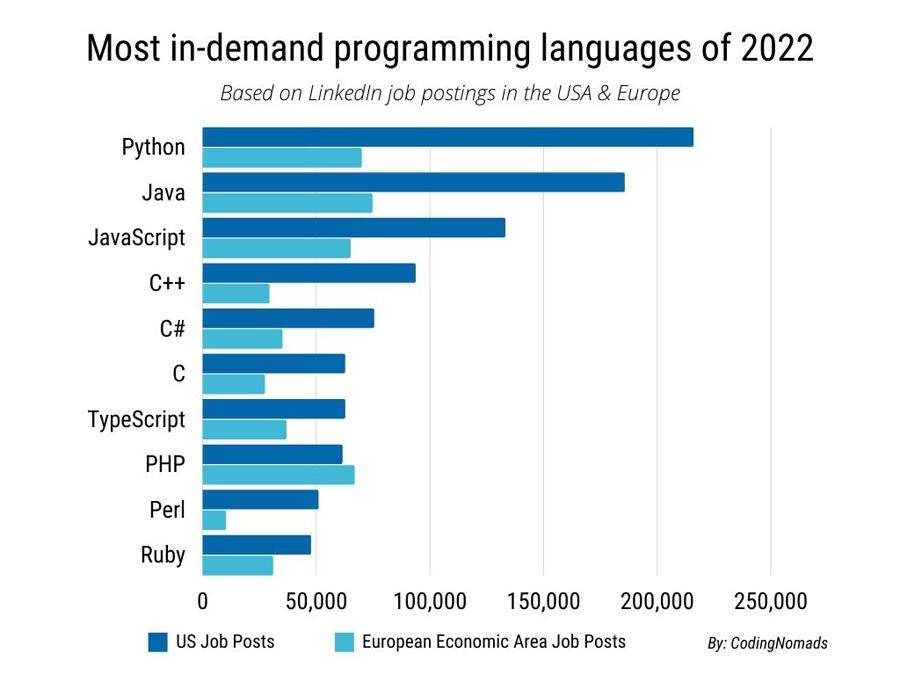
\includegraphics[scale=0.3]{figures/most-in-demand-programming-languages-of-2022-codingnomads.jpg}
  \caption[]{An example chart showing the change of popularity of
    various programming languages, taken from techrepublic Website\footnotemark[1].}
  \label{fig:example}
\end{figure}

\footnotetext[1]{\url{https://www.techrepublic.com/article/the-best-programming-languages-to-learn-in-2022/}}

In the Latex source provided together with this PDF, you also find hints on how to work on one Latex project collaboratively.


%%%%%%%%%%%%%%%%%%%%%%%%%%%%%%%%%%%%%%%%%%%%%%%%%%%%%%%%%%%%

% The following is especially useful if you work together on one proposal or report, and want to alter its content independently from each other (e.g., to keep your commit history clean).

% Alternative: put content in separate files
% Check the difference between including these files using \input{filename} and \include{filename} and see which one you like better
%\chapter{Einleitung}\label{intro}
%\input{introduction}
%
%\chapter{Voraussetzungen}\label{bg}
%\input{background}

%%%%%%%%%%%%%%%%%%%%%%%%%%%%%%%%%%%%%%%%%%%%%%%%%%%%%%%%%%%%

% References (Literaturverzeichnis):
% see
% https://de.wikibooks.org/wiki/LaTeX-W%C3%B6rterbuch:_bibliographystyle
% for the different formats and styles

\bibliographystyle{plain}
% b) The File:
\bibliography{references}

\end{document}
